\documentclass[english,,man]{apa6}
\usepackage{lmodern}
\usepackage{amssymb,amsmath}
\usepackage{ifxetex,ifluatex}
\usepackage{fixltx2e} % provides \textsubscript
\ifnum 0\ifxetex 1\fi\ifluatex 1\fi=0 % if pdftex
  \usepackage[T1]{fontenc}
  \usepackage[utf8]{inputenc}
\else % if luatex or xelatex
  \ifxetex
    \usepackage{mathspec}
  \else
    \usepackage{fontspec}
  \fi
  \defaultfontfeatures{Ligatures=TeX,Scale=MatchLowercase}
\fi
% use upquote if available, for straight quotes in verbatim environments
\IfFileExists{upquote.sty}{\usepackage{upquote}}{}
% use microtype if available
\IfFileExists{microtype.sty}{%
\usepackage{microtype}
\UseMicrotypeSet[protrusion]{basicmath} % disable protrusion for tt fonts
}{}
\usepackage{hyperref}
\hypersetup{unicode=true,
            pdftitle={Inferences With Longitudinal Data},
            pdfauthor={Christopher R. Dishop, Mike Braun, Goran Kuljanin, \& Richard P. DeShon},
            pdfkeywords={Inferences, dynamics, growth, longitudinal, process, over time, tvc,
hlm, sem, models},
            pdfborder={0 0 0},
            breaklinks=true}
\urlstyle{same}  % don't use monospace font for urls
\ifnum 0\ifxetex 1\fi\ifluatex 1\fi=0 % if pdftex
  \usepackage[shorthands=off,main=english]{babel}
\else
  \usepackage{polyglossia}
  \setmainlanguage[]{english}
\fi
\usepackage{graphicx,grffile}
\makeatletter
\def\maxwidth{\ifdim\Gin@nat@width>\linewidth\linewidth\else\Gin@nat@width\fi}
\def\maxheight{\ifdim\Gin@nat@height>\textheight\textheight\else\Gin@nat@height\fi}
\makeatother
% Scale images if necessary, so that they will not overflow the page
% margins by default, and it is still possible to overwrite the defaults
% using explicit options in \includegraphics[width, height, ...]{}
\setkeys{Gin}{width=\maxwidth,height=\maxheight,keepaspectratio}
\IfFileExists{parskip.sty}{%
\usepackage{parskip}
}{% else
\setlength{\parindent}{0pt}
\setlength{\parskip}{6pt plus 2pt minus 1pt}
}
\setlength{\emergencystretch}{3em}  % prevent overfull lines
\providecommand{\tightlist}{%
  \setlength{\itemsep}{0pt}\setlength{\parskip}{0pt}}
\setcounter{secnumdepth}{0}
% Redefines (sub)paragraphs to behave more like sections
\ifx\paragraph\undefined\else
\let\oldparagraph\paragraph
\renewcommand{\paragraph}[1]{\oldparagraph{#1}\mbox{}}
\fi
\ifx\subparagraph\undefined\else
\let\oldsubparagraph\subparagraph
\renewcommand{\subparagraph}[1]{\oldsubparagraph{#1}\mbox{}}
\fi

%%% Use protect on footnotes to avoid problems with footnotes in titles
\let\rmarkdownfootnote\footnote%
\def\footnote{\protect\rmarkdownfootnote}


  \title{Inferences With Longitudinal Data}
    \author{Christopher R. Dishop\textsuperscript{1}, Mike Braun\textsuperscript{2},
Goran Kuljanin\textsuperscript{3}, \& Richard P.
DeShon\textsuperscript{1}}
    \date{}
  
\shorttitle{LONGITUDINAL INFERENCES}
\affiliation{
\vspace{0.5cm}
\textsuperscript{1} Michigan State University\\\textsuperscript{2} University of South Florida\\\textsuperscript{3} DePaul University}
\keywords{Inferences, dynamics, growth, longitudinal, process, over time, tvc, hlm, sem, models\newline\indent Word count: 95}
\usepackage{csquotes}
\usepackage{upgreek}
\captionsetup{font=singlespacing,justification=justified}

\usepackage{longtable}
\usepackage{lscape}
\usepackage{multirow}
\usepackage{tabularx}
\usepackage[flushleft]{threeparttable}
\usepackage{threeparttablex}

\newenvironment{lltable}{\begin{landscape}\begin{center}\begin{ThreePartTable}}{\end{ThreePartTable}\end{center}\end{landscape}}

\makeatletter
\newcommand\LastLTentrywidth{1em}
\newlength\longtablewidth
\setlength{\longtablewidth}{1in}
\newcommand{\getlongtablewidth}{\begingroup \ifcsname LT@\roman{LT@tables}\endcsname \global\longtablewidth=0pt \renewcommand{\LT@entry}[2]{\global\advance\longtablewidth by ##2\relax\gdef\LastLTentrywidth{##2}}\@nameuse{LT@\roman{LT@tables}} \fi \endgroup}


\DeclareDelayedFloatFlavor{ThreePartTable}{table}
\DeclareDelayedFloatFlavor{lltable}{table}
\DeclareDelayedFloatFlavor*{longtable}{table}
\makeatletter
\renewcommand{\efloat@iwrite}[1]{\immediate\expandafter\protected@write\csname efloat@post#1\endcsname{}}
\makeatother
\usepackage{lineno}

\linenumbers

\authornote{\ldots{}.

Correspondence concerning this article should be addressed to
Christopher R. Dishop, 316 Physics Road, Psychology Building, Room 348,
East Lansing, MI, 48823. E-mail:
\href{mailto:dishopch@msu.edu}{\nolinkurl{dishopch@msu.edu}}}

\abstract{
Our field is increasingly interested in how things that happen over
time, in within-person phenomena, dynamics, growth, person-oriented
frameworks, and fundamental patterns in longitudinal data structures.
Longitudinal data structures lend themselves to many different
inferences -- to different patterns that researchers may emphasize --
and there are different statistical models available for anyone armed
with repeated measures. Although the diversity of inferences and models
provides a wide foundation for exploring a content area, it can also
make it difficult for researchers to know all of the inferences
available to them, which models to evoke given their question, and how
to locate their specific study within the broader set of ``over time''
inferences. We developed a framework that situates these inferences into
a core set that exposes researchers to the variety of questions and
inferences that can explore with longitudinal data. In this paper we
unpack that framework, discuss the inferences, and link every inference
to a set of models so that researchers know where to turn given their
specific interest.


}

\usepackage{amsthm}
\newtheorem{theorem}{Theorem}[section]
\newtheorem{lemma}{Lemma}[section]
\theoremstyle{definition}
\newtheorem{definition}{Definition}[section]
\newtheorem{corollary}{Corollary}[section]
\newtheorem{proposition}{Proposition}[section]
\theoremstyle{definition}
\newtheorem{example}{Example}[section]
\theoremstyle{definition}
\newtheorem{exercise}{Exercise}[section]
\theoremstyle{remark}
\newtheorem*{remark}{Remark}
\newtheorem*{solution}{Solution}
\begin{document}
\maketitle

Organizational phenomena unfold over time. They are processes that
develop, change, and evolve (Pitariu \& Ployhart, 2010) that create a
sequence of events within a person's stream of experience (Beal, 2015).
Moreover, organizations are systems with many connected parts, and
systems are inherently dynamic. Studying these systems and processes,
therefore, requires that we attend not to static snapshots of behavior
(Ilgen \& Hulin, 2000), but to variables and relationships as they move
through time; doing so puts us in a better position to capture the
sequence, understand it, and can lead to new and interesting insights
(Kozlowski \& Bell, 2003).

We have noticed a variety of inferences emerging in our literature that
researchers explore when they want to understand something over time.
Some focus on whether trajectories increase or decrease, or the pattern
of growth in a variable over time. Others turn their attention not to
trends but to relationship patterns across time. There is also an
increasing emphasis on dynamics. How are these ways of asking questions
about patterns in longitudinal data different? We find these inferences
everywhere, and their persistence has driven us to ask how to organize
them.

We developed a framework to capture these inferences; a way to organize
the fundemental patterns researchers explore with longitudinal data
despite focusing on different content areas or using different
statistical models. Often research groups focus on one familiar
inference despite having the data to explore many more fundamental
patterns. There are also a number of complex statistical models
lingering in our literature, and it is not always clear for which
questions they are appropriate. We want to be sure researchers have a
framework to expose the core patterns in longitudinal data as these data
structures become more popular in our field.

In this paper we discuss the common inferences that researchers in our
field make when they apply a model to longitudinal data. As should be
clear to anyone reading our literature, there is great excitement for
the utility of longitudinal studies; they can pose interesting questions
and discover patterns that would otherwise be impossible to capture in a
static investigation. We bring attention to the span of questions
available so that researchers can fully appreciate and take advantage of
their data. Although the inferences all concern trajectories over time,
their small differences have large implications for what we take away
from them -- what we ultimately conclude. Moreover, there are many
inferences, many models, and different models can be used to understand
or explore the same inference. In this paper, we provide readers with
potential models for each inference so that they can be sure that the
model they evoke is appropriate for the research question that they are
interested in. In summary, this paper exposes researchers to the span of
inferences they may investigate when they collect longitudinal data,
links those inferences to models, and parses some of the modeling
literature that may be difficult to consume for researchers with only
graduate level training in statistics.

\hypertarget{longitudinal-definitions}{%
\section{Longitudinal Definitions}\label{longitudinal-definitions}}

This paper is exclusively devoted to the inferences we make with
repeated observations, so we begin by identifying a few labels and
definitions. Authors typically identify a \enquote{longitudinal} study
by contrasting either (a) research designs or (b) data structures.
Longitudinal \emph{research} is different from cross-sectional research
because longitudinal designs entail three or more repeated observations
(Ployhart \& Vandenberg, 2010). We therefore emphasize differences on
the number of observations when we distinguish longitudinal from other
types of research. Longitudinal \emph{data} are repeated observations on
several units (i.e., \(N\) or \(i\) \textgreater{} 1), whereas panel
data are observations of one unit over time -- a distinction that
focuses on the amount of people in our study (given repeated measures).
Most organizational studies collect data on more than one unit,
therefore our discussion below focuses on longitudinal research with
longitudinal data, or designs with \(N\) \textgreater{} 1, \(t\)
\textgreater{}= 3, and the same construct(s) measured on each \(i\) at
each \(t\). In English, we focus on designs that measure their variables
repeatedly across many people -- and every variable is measured at each
time point.

\hypertarget{framework}{%
\section{Framework}\label{framework}}

We use four inference categories to partition our discussion, including
level, trend, relationships, and dynamics. Each of these are broad
categories, and they will all have their own sub-inferences and models.
Our writing style will be the same throughout each section, where we
first discuss the category itself and then sequentially walk through the
inferences. During that sequence, we will pose questions to orient the
reader as to what the inference captures, unpack graphs and figures, and
then close with a table that provides example hypotheses that align with
each inference. The figures we use in the level, trend, and
relationships sections are graphs that show what the inferences look
like in data -- we feel that graphing the inferences with respect to
data is more informative than your usual box and arrow diagram. There is
a caveat, however, that we want to make sure everyone is aware of. Data
are always messy. It is rare to find data where the inferences expose
themselves simply by plotting -- although it is certainly possible. We
are using these \enquote{data plots} to clearly convey what the
inferences mean, but please be aware that field data will always be
messy. When we discuss dynamics we then use box and arrow diagrams
because they better convey the ideas in that section.

Finally, we end each inference section by pointing researchers to
respective statistical models. Although we direct researchers to models,
our paper is not about statistical modeling only -- it is about
inferences -- and researchers therefore need to be sure that they
appreciate all of the nuance before applying a recommended model. There
are many complex statistical issues that arise with longitudinal
modeling -- like stationarity -- and the models differ in how they
handle these issues, the assumptions they make, and the data format they
require. There are plenty of great references on each model, what we are
doing here is guiding researchers to those references based on the
underlying inferences that interest them.

\hypertarget{level}{%
\section{Level}\label{level}}

Is employee emotional exhaustion, on average, high across the study? Is
trainee skill low at the beginning of a training session? What value are
newcomer perceptions of unit climate at the end of a two-week
socialization process? These are questions about level, or the specific
value of a variable.

\hypertarget{comment}{%
\subsubsection{Comment}\label{comment}}

Some comment here.

Levels either describe the variable at one moment or averaged across a
span of time. That is, if we put a variable on the \(y\) axis and plot
its values against time on the \(x\) axis, we can explore the value that
it takes at time \(t\), or the value that it takes on average across any
span of \(t\).

Figure \ref{level} demonstrates this idea graphically. A variable is
plotted across time for a single person (i.e., unit), and the color
labels indicate levels -- the red and green describe the variable at a
specific moment while the purple, average level, describes it across a
window. The starting level is the value of the variable at the first
time point, the ending level is its value at the last time point, and
the average level is its average level across time.

\begin{center}

------------

Insert Figure \ref{level} about here

------------

\end{center}

\noindent Our first level inference, therefore, concerns the value of a
variable at a specific time or averaged across a window of time.

\begin{quote}
\begin{quote}
\textbf{Inference 1:} What is the level of \(x\) at time \(t\), or
across a span of \(t\)?
\end{quote}
\end{quote}

When we retain one variable but add multiple units -- people or
organizations, for example -- then we can examine variability in level.
Does everyone have high affect across time? Is there variability in the
level of skill among trainees at the beginning of a training session?

We demonstrate this idea in figure \ref{level_var}, where we now plot
three units (people) across time. Each individual has a similar
trajectory, but their ending levels of \(y\) are different. Said
formally that is, \enquote{there is variability across units in level at
the last time point.}

\begin{center}

------------

Insert Figure \ref{level_var} about here

------------

\end{center}

\noindent The second level inference, therefore, is about level
variability across units.

\begin{quote}
\begin{quote}
\textbf{Inference 2:} Across a span of \(t\) or at a specific \(t\)
there is variability in the level of \(x\).
\end{quote}
\end{quote}

Inferences one and two concern a single variable, but they can of course
be iterated across any or all observed variables in the study (remember
that variables are different than units). For example, we might discover
that affect and performance have high average levels across time, but
that affect has greater level variability across units. Or we might
learn that affect has a low initial level whereas performance is
initially high. What we are doing here is making descriptive comparisons
between the level of one variable and the level of another. We can also
produce a quantitative statement about the extent to which levels are
related.

Correlating levels provides us with that quantitative statement. A large
positive correlation between the initial levels of affect and
performance would mean that people with greater initial levels of affect
also tend to have greater intial performance, and people with lower
initial affect also tend to have lower initial performance.

Figure \ref{level_correlate} demonstrates a correlation of starting
levels. In Panel A we plot affect and performance trajectories for three
individuals across time, where the black solid line indicates affect and
the dashed line indicates performance. We indicate starting levels for
both variables in Panel A by placing colored circles on the graph for
each individual. For example, we indicate the starting levels of affect
and performance for person one with red circles and the starting levels
for person two with green circles.

Panel B of figure \ref{level_correlate} maps those starting levels onto
a new plot that leads to our inference. On the \(x\)-axis is initial
level of affect where high values indicate a high starting level of
affect, and on the \(y\)-axis is initial level of performance where high
values indicate a high starting level of performance. The red circle for
person one is on the bottom right because that individual has a high
initial level of affect and a low initial level of performance. Person
two (the green circle) is on the top left because that individual has a
high initial level of performance and a low initial level of affect, and
person three is in the middle because they have roughly the same
starting levels of affect and performance. The dots slope downward in
Panel B, which tells us that there is a negative relationship between
initial level of affect and initial level of performance.

Overall, figure \ref{level_correlate} suggests that the starting levels
of affect and performance are correlated. Panel A shows the actual
starting levels, and Panel B shows that there is a strong negative
correlation between initial affect and initial performance. This
negative relationship means that we expect people with low initial
affect to have high initial performance, whereas we expect people with
high initial affect to have low initial performance.

\begin{quote}
\begin{quote}
\textbf{Inference 3:} There is a correlation between the level of \(x\)
and the level of \(y\) at \(t\).
\end{quote}
\end{quote}

\begin{center}

------------

Insert Figure \ref{level_correlate} about here

------------

\end{center}

\hypertarget{level-inference-table}{%
\subsection{Level Inference Table}\label{level-inference-table}}

The inference table below provides examples of each level inference.
Inference one is about level itself -- a single value that describes the
variable at one time or averaged across time. Inference two is about
variability across units in level. Inference three takes the level in
one variable and asks whether it tends to co-occur with the level in
another. Think of inference three as creating a latent level variable at
a single moment and asking how it relates to another latent variable
from a single moment.

\begin{center}

------------

Insert Table \ref{level_table} about here

------------

\end{center}

\hypertarget{models}{%
\subsection{Models}\label{models}}

Level is called the intercept in the statistical modeling literature.
That is, when a researcher estimates a model to explore the starting
level of a variable, like performance, she is estimating the intercept
at the initial time point. The analysis will return a mean estimate
which tells you about level, and it will also return a variance estimate
that indicates variability across units. Typically you will hear
researchers refer to models that only explore level as intercept-only
models. Intercept-only models are almost always paired with more complex
growth models, so we will save our reference recommendations for the
next section. If a researcher is interested in level he or she can look
to the references we point to in the next, \enquote{trend} section, all
of those models also examine intercepts.

\begin{table}

\caption{\label{tab:unnamed-chunk-7}\label{level_table}Examples of level inferences.}
\centering
\begin{tabular}[t]{>{\raggedright\arraybackslash}p{5em}>{\raggedright\arraybackslash}p{30em}}
\toprule
Inference & Examples\\
\midrule
1 & Burnout is high at the last time point.\newline Performance is low, on average, across time.\\
\hline
2 & Average affect across time differs across people (units).\newline There is variability in the initial level of turnover across organizations.\\
\hline
3 & People with greater initial health status also have greater initial happiness.\newline People with high performance on average across time have lower anxiety on average across time.\\
\bottomrule
\end{tabular}
\end{table}

\begin{figure}
\centering
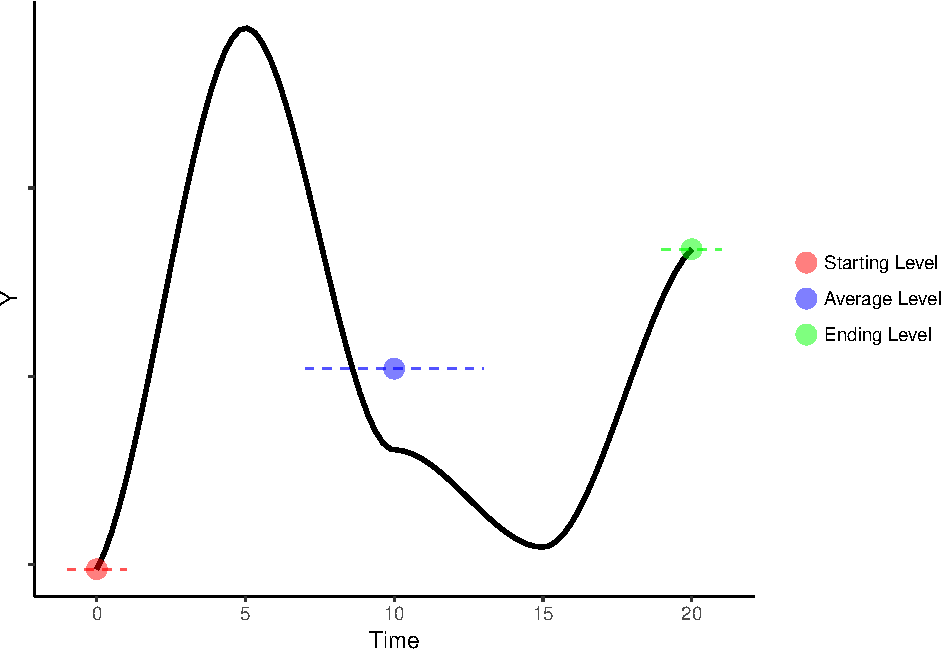
\includegraphics{figures/unnamed-chunk-8-1.pdf}
\caption{\label{fig:unnamed-chunk-8}Level examples.\label{level}}
\end{figure}

\begin{figure}
\centering
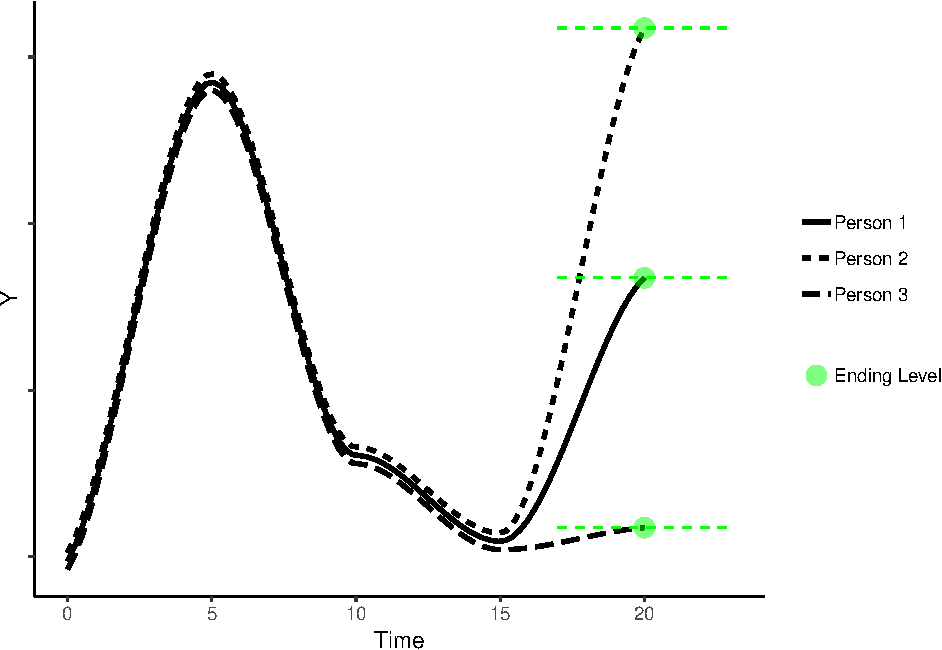
\includegraphics{figures/unnamed-chunk-9-1.pdf}
\caption{\label{fig:unnamed-chunk-9}Trajectories with variability in ending
level across units.\label{level_var}}
\end{figure}

\begin{figure}
\centering
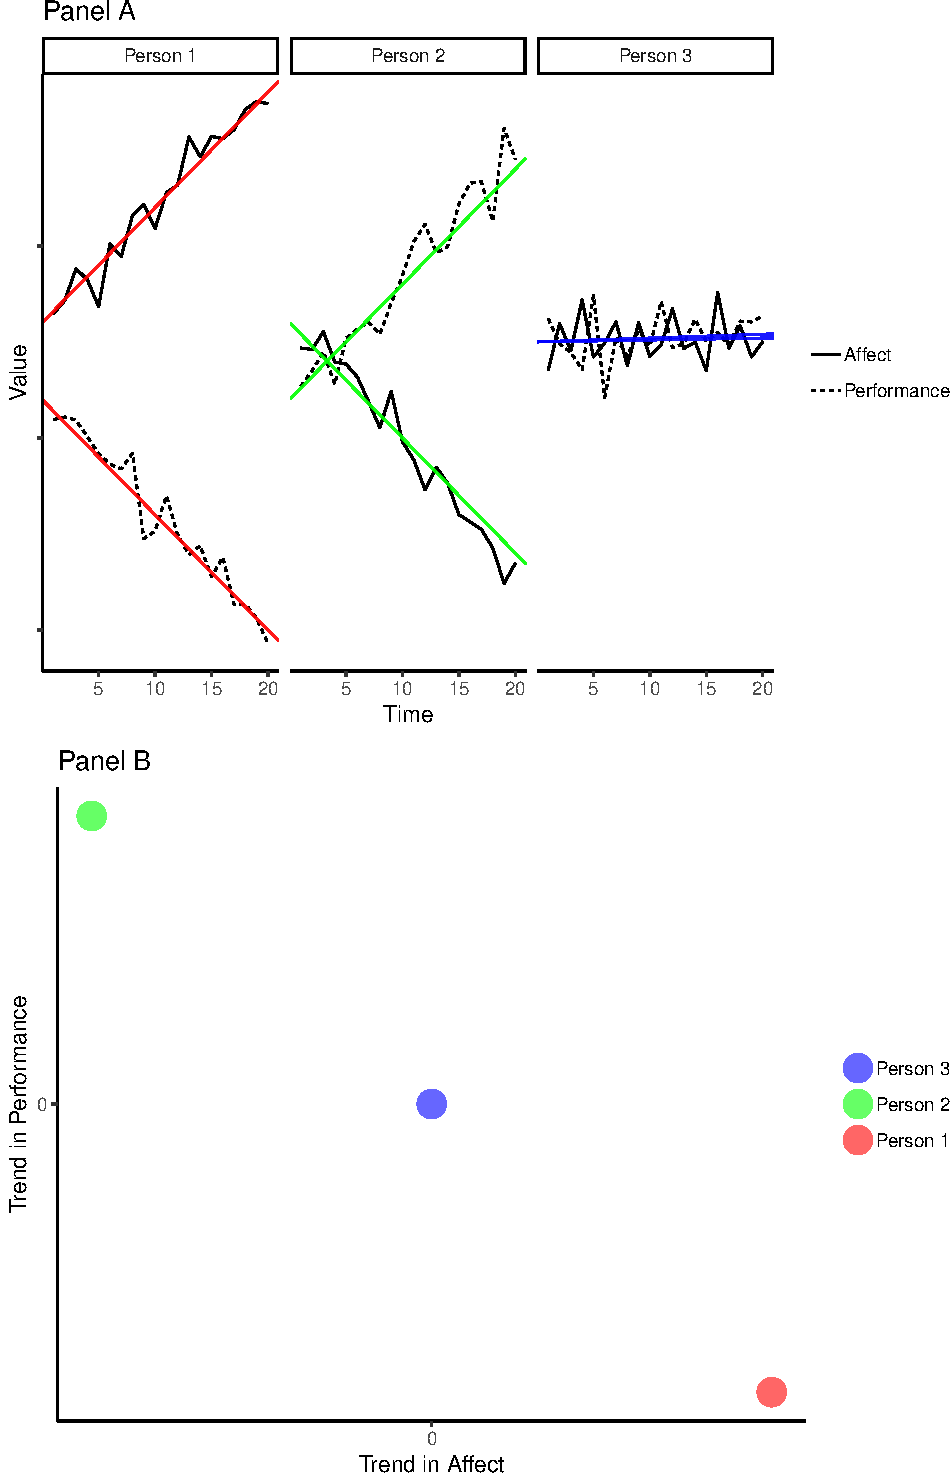
\includegraphics{figures/unnamed-chunk-10-1.pdf}
\caption{\label{fig:unnamed-chunk-10}Correlating starting levels, or
relating initial affect to initial performance.\label{level_correlate}}
\end{figure}

\hypertarget{trend}{%
\section{Trend}\label{trend}}

Does affect go up or down across time, or is it relatively stable? Does
trainee skill increase over the training session? These are questions
about trend, and these first two are specifically about linear trend. It
is also possible to explore how variables bend or curve across time. Do
newcomer perceptions of climate increase and then plateau over time?
Does the response time of a medical team decrease with each successive
case but then remain stable once the team can no longer improve their
coordination? These latter questions concern curvilinear trajectories.

Trend has to do with the global shape of the trajectory across time. If
we put a variable on the \(y\)-axis and plot its values against time on
the \(x\)-axis, do the values tend to go up or down over time? It can be
thought of as the coarse-grained direction of a trajectory.

Figure \ref{trend} demonstrates trend, where the red line shows
negative, decreasing trend, the blue line shows positive, increasing
trend, and the green line shows a curvilinear trajectory. Keep in mind
that curvilinear and linear trajectories are both \emph{linear in
parameters} and should not be confused with non-linear systems.

\begin{center}

------------

Insert Figure \ref{trend} about here

------------

\end{center}

Our first trend inference, therefore, concerns the shape of the
trajectory.

\begin{quote}
\begin{quote}
\textbf{Inference 1:} There is positive/negative/curvilinear trend in a
variable across time.
\end{quote}
\end{quote}

As with the level inferences, when we add more units we can examine
trend variability. Do all trainees develop greater skill across time? Is
there variability in the trend of helping behaviors, or
counterproductive work behaviors over time?

Figure \ref{trend_var} shows differences in trend variability. In the
first facet all units (people) show the same positive trend, whereas
everyone in the second facet shows different trend: person one's data
appear to increase over time, person two's data decrease over time, and
person three's data remain flat. With greater variability there is less
consistency in trend across units.

\begin{center}

------------

Insert Figure \ref{trend_var} about here

------------

\end{center}

\begin{quote}
\begin{quote}
\textbf{Inference 2:} Trend differs/does not differ across units.
\end{quote}
\end{quote}

Inferences one and two are about one variable, but they can also be
iterated across all observed variables. For example, we might discover
that affect and performance trends both decrease, but there is greater
variability across units in the affect trend. Or we might learn that
affect has a negative trend while performance has a positive trend.

Correlating these trends is the next inference. Correlating indicates
co-occuring patterns, but this time we focus on trends rather than
levels. A large positive correlation between affect and performance
trends indicates that people with a positive affect trend (usually) have
a positive performance trend and people with a negative affect trend
(usually) have a negative performance trend.

Figure \ref{trend_correlation} shows the inuition behind the inference
with a set of graphs. In Panel A we plot affect and performance across
time for three individuals. Affect goes up while performance goes down
for person one, this pattern is reversed for person two, and person
three reports trendless affect and performance (i.e., zero trend), but
both variables fluctuate across time for this individual. We use
different colors to label the trends for each person. The affect and
performance trends for person one are labeled with red lines, whereas
person two has green lines and person three has blue lines.

Panel B then maps those pairings onto a figure that shows the
relationship between the affect and performance trend. For example,
person one has a positive affect trend and a negative performance trend,
so their value in Panel B goes on the bottom right, whereas person two
has the opposite pattern and therefore is placed on the top left (where
the performance trend is positive and the affect trend is negative).
Producing this bottom scatter plot tells us that the relationship
between the affect and performance trend is negative. That is, people
with a positive affect trend usually have a negative performance trend,
people with a negative affect trend are more likely to have a positive
performance trend, and people with no affect trend usually have no
performance trend.

\begin{center}

------------

Insert Figure \ref{trend_correlation} about here

------------

\end{center}

\begin{quote}
\begin{quote}
\textbf{Inference 3:} There are correlated trends.
\end{quote}
\end{quote}

The final trend inference is about identifying covariates or predictors
of trend. Does gender predict depletion trends? Does the trend in unit
climate covary with between unit differences in leader quality? Notice
the difference between this inference and inference three. Inference
three asks how one trend is related to another, whereas this inference
asks how one trend relates to a covariate.

Figure \ref{trend_covariate} demonstrates the inference in a plot. We
plot affect across time for six employees, and these employees differ by
job type. The first three individuals work in research and development,
whereas the final three individuals work in sales. Affect trajectories
tend to decrease over time for employees in research and development,
whereas affect trajectories tend to increase for those in sales. An
individual's job type, then, gives us a clue to their likely affect
trend -- said formally, job type covaries with affect trends, such that
we expect individuals in sales to have positive affect trends and
individuals in research and development to have negative affect trends.
The expected trends are plotted as the thick blue lines.

\begin{center}

------------

Insert Figure \ref{trend_covariate} about here

------------

\end{center}

\begin{quote}
\begin{quote}
\textbf{Inference 4:} There are correlates of trend.
\end{quote}
\end{quote}

\hypertarget{trend-inference-table}{%
\subsection{Trend Inference Table}\label{trend-inference-table}}

The inference table below provides examples of each trend inference.
Inference one is about the general direction or shape of a trajectory
across time. Inference two is about variability in that shape across
units. Inference three takes the trend in one variable and asks whether
it co-occurs with trend in another. Inference four, finally, is about
the relationship between trend in one variable and the raw values of one
or more correlates.

\begin{center}

------------

Insert Table \ref{trend_table} about here

------------

\end{center}

We want to close this section with a note on phrasing. The inferences we
explored in this section have to do with correlating trends, where a
statement like \enquote{affect and performance trends covary, such that
people with a negative affect trend have a positive performance trend}
is appropriate. There is a less precise phrase that is easy to fall into
-- and we have seen it used in our literature. Sometimes, researchers
will correlate trends and then state, \enquote{when affect decreases
performance goes up.} We urge researchers to avoid this second statement
because it is not clear if it refers to a static relationship about
trends or a dynamic statement about how trajectories move across time.
That is, the phrase \enquote{when affect decreases performance goes up}
could refer to correlated trends, but it could also mean something like,
\enquote{when affect decreases performance immediately or subsequently
goes up.} This second statement is far different and it should not be
used when an analysis only correlates trends or evokes predictors of
trend. Again, we urge researchers to phrase their inferences as we have
shown here.

\hypertarget{models-1}{%
\subsection{Models}\label{models-1}}

Trend is called the slope in the statistical modeling literature. That
is, when a researcher estimates a model to explore whether a variable
goes up or down over time she is estimating the trend coefficient.
Again, the mean estimate will tell you about the trend itself and the
variance estimate refers to the trend variability across units. In the
statistical modeling literature these models are called growth-models or
growth-curves. Keep in mind, however, that researchers use the word
\enquote{change} informally to mean growth as well, so when you read a
theoretical discussion you may see words like \enquote{change} and
\enquote{increase} despite the researcher using a \enquote{growth}
model.

Broad theoretical discussions of growth and change are found in Pitariu
and Ployhart (2010) and Ployhart and Vandenberg (2010), whereas Bliese
and Ployhart (2002) describe how to go about running an analysis. Growth
curves are a core topic in developmental psychology, so there are many
great articles and textbooks to read from their field. See Grimm, Ram,
and Estabrook (2016) and Singer, Willett, and Willett (2003) for two
great textbooks on growth curve modeling, and McArdle and Epstein (1987)
for an empirical discussion. For two straight-forward empirical examples
in our own field see Dunford, Shipp, Boss, Angermeier, and Boss (2012)
and Hülsheger (2016).

\begin{table}

\caption{\label{tab:unnamed-chunk-11}\label{trend_table}Examples of trend inferences.}
\centering
\begin{tabular}[t]{>{\raggedright\arraybackslash}p{5em}>{\raggedright\arraybackslash}p{30em}}
\toprule
Inference & Examples\\
\midrule
1 & Burnout decreases over time.\newline Performance increases over time.\\
\hline
2 & Affect trends differ across people (units).\newline There is variability in turnover trends across organizations.\\
\hline
3 & People with a positive health status trend have a positive happiness trend.\newline People with a positive performance trend have a negative anxiety trend.\\
\hline
4 & Gender correlates with depletion trends.\newline Unit climate covaries with unit performance trends.\\
\bottomrule
\end{tabular}
\end{table}

\begin{figure}
\centering
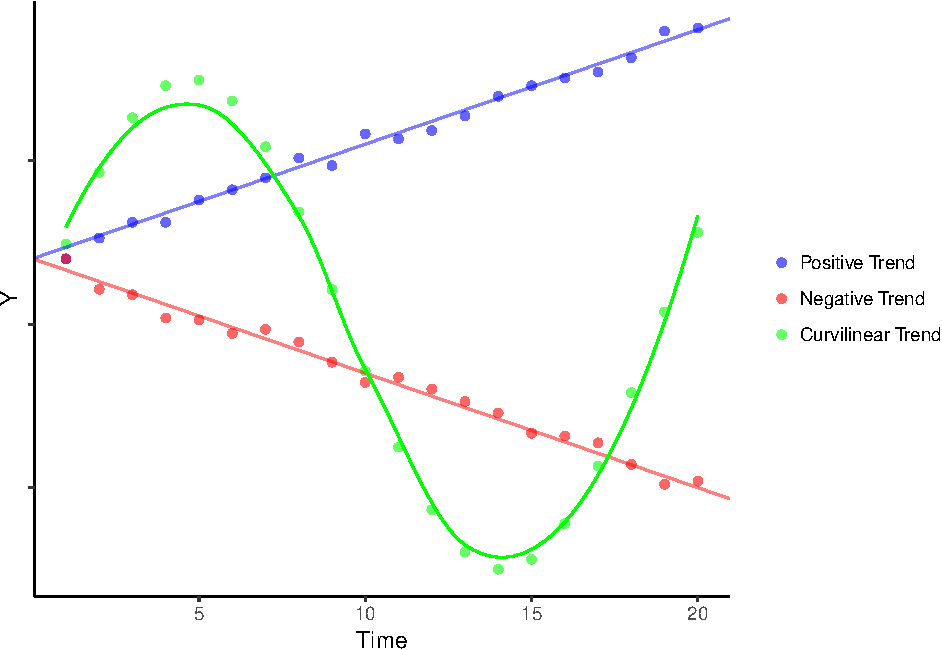
\includegraphics{figures/unnamed-chunk-12-1.pdf}
\caption{\label{fig:unnamed-chunk-12}Trend across time.\label{trend}}
\end{figure}

\begin{figure}
\centering
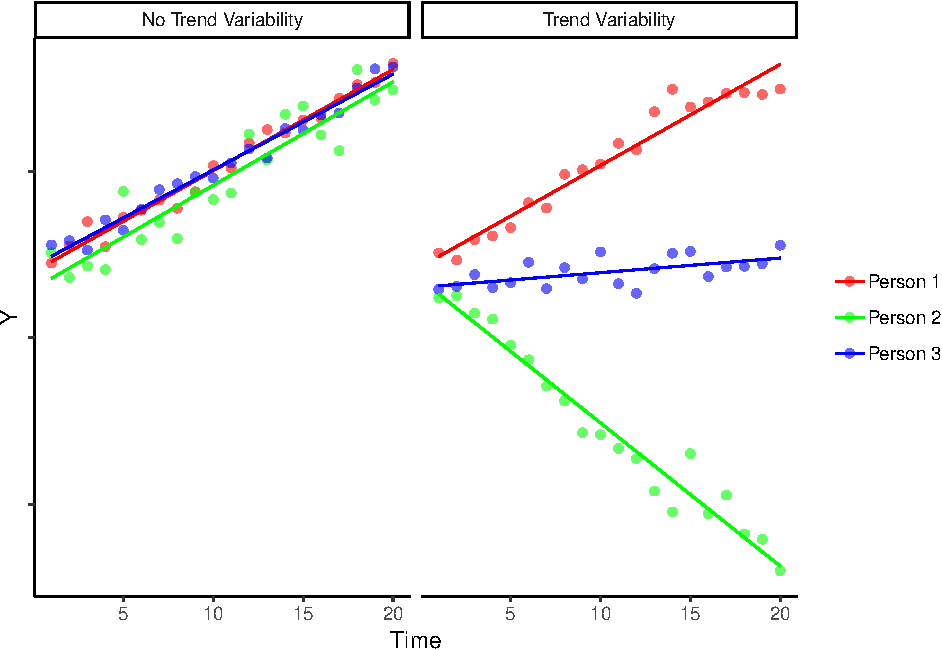
\includegraphics{figures/unnamed-chunk-13-1.pdf}
\caption{\label{fig:unnamed-chunk-13}Differences in trend variability across
units.\label{trend_var}}
\end{figure}

\begin{figure}
\centering
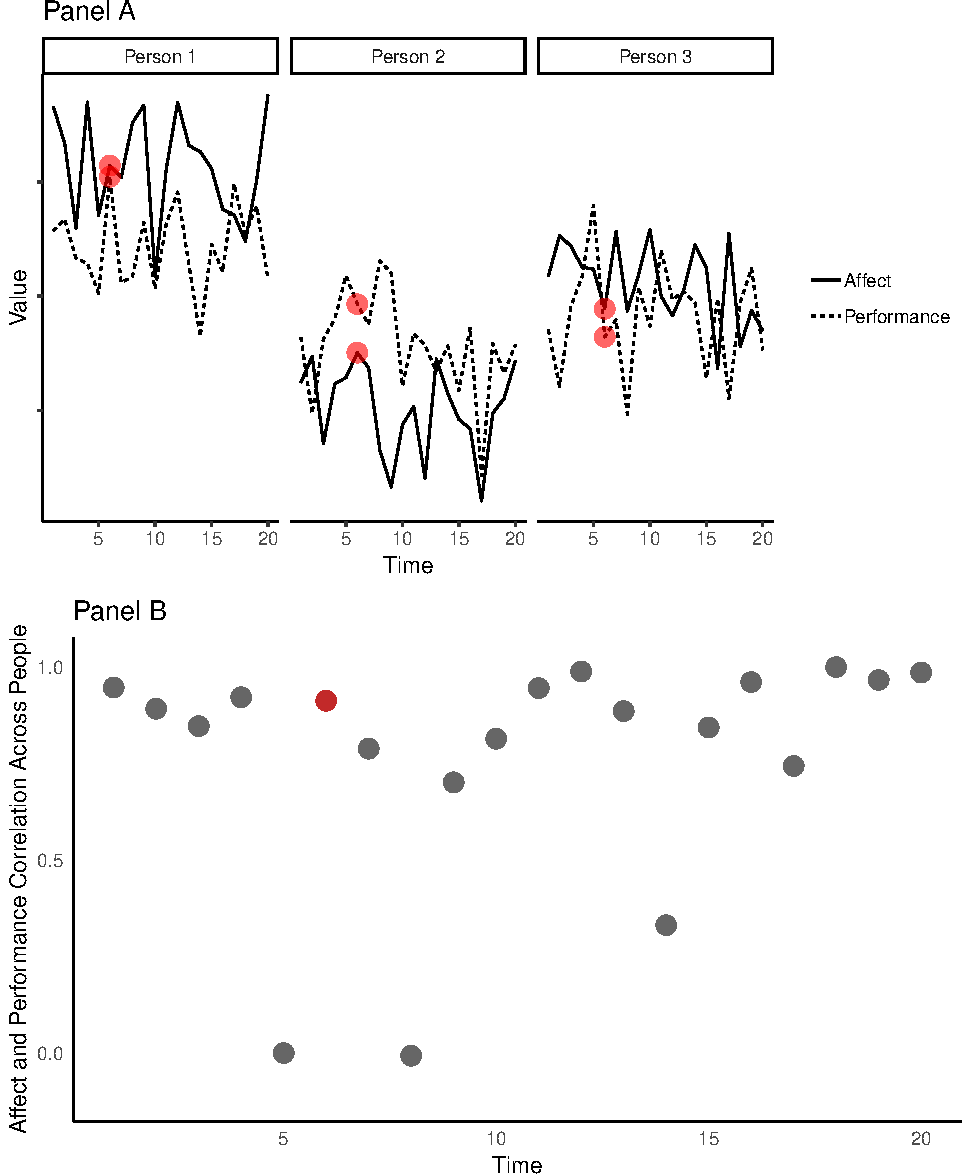
\includegraphics{figures/unnamed-chunk-14-1.pdf}
\caption{\label{fig:unnamed-chunk-14}Correlating slopes, or relating the
affect to performance trend.\label{trend_correlation}}
\end{figure}

\begin{figure}
\centering
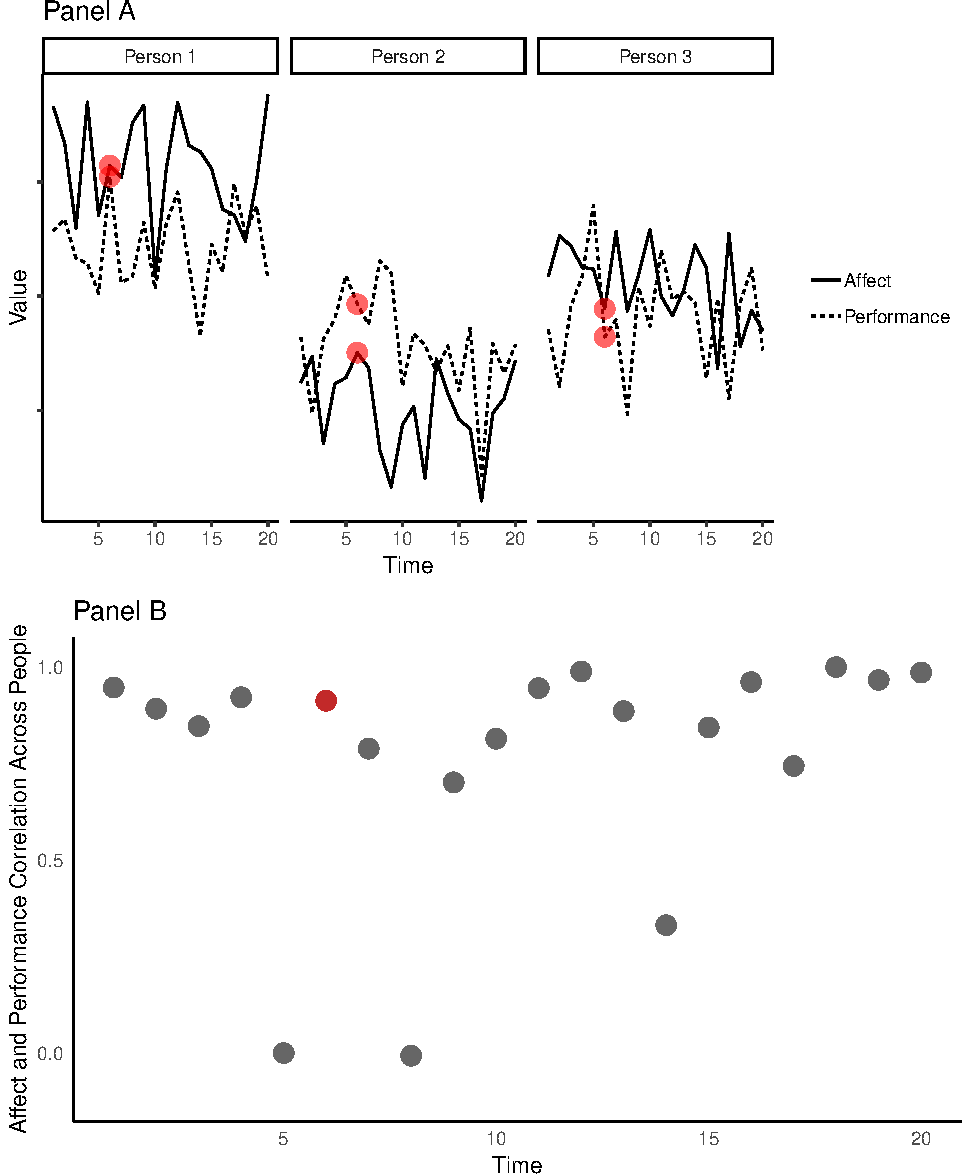
\includegraphics{figures/unnamed-chunk-15-1.pdf}
\caption{\label{fig:unnamed-chunk-15}Job type as a covariate of affect
trend.\label{trend_covariate}}
\end{figure}

\hypertarget{relationships}{%
\section{Relationships}\label{relationships}}

In the sections above we explored covariance at a single moment, general
trends, and covariance between trends. Here, we explore relationship
patterns between two variables over time. Does affect relate to
performance across time? Over time, does unit climate covary with shared
mental models? Do the fluctuations in voice match the fluctuations in
commitment over time -- i.e., when voice is high is commitment also
high?

Our first inference focuses on a single unit -- one person, one team, or
one organization over time. The trajectory of a single unit over time is
called a time-series, and two are plotted simultaneously in figure
\ref{relation_ts}. The solid line shows a time-series of affect over
time, and the dashed line plots a time-series of performance. Notice
that, across time, when affect is high respective to itself performance
is also high (and vice versa). The colored squares represent values of
each variable at different points in time. The green squares highlight
low values of both variables, the blue high values, and the red middle
values.

\begin{center}

------------

Insert Figure \ref{relation_ts} about here

------------

\end{center}

Panel B shows how those respective values map onto a scatterplot of
affect and performance -- which again will lead to the inference. The
blue values indicate that high values of affect tend to co-occur with
high values of performance (shown respectively by the blue squares in
Panel A). The red values indicate that middle values of affect tend to
co-occur with middle values of performance. The green values, finally,
indicate that low values of affect tend to co-occur with low values of
performance. Across time, affect and performance covary and the
relationship is positive.

\begin{quote}
\begin{quote}
\textbf{Inference 1:} There is a relationship between \(x\) and \(y\)
across time.
\end{quote}
\end{quote}

What happens when we add more units? Doing so changes the question from
\enquote{what is the relationship across time} to, \enquote{at each
moment, what is the relationship across units?} Ultimately we move from
a within-unit question to a between-unit focus, and we apply that
between unit focus to each time point.

In the prior inference we asked if affect relates to performance across
time -- on a single person/unit. Now imagine that we gather data on
multiple people across time, so we have many affect and performance
trajectories. One of the most popular inferences in our literature is to
take those time series and slice them into individual time points, look
at between-person correlations among affect and performance at a single
moment, and then repeat that analysis for each time point. At time one,
what is the correlation between affect and performance? At time two,
what is the correlation between affect and performance? At time three,
what is the correlation between affect and performance? Because we have
multiple people we can explore correlations at a single moment.
Researchers then typically report the average of these single moment
correlations, or they constrain them to be equal across time.

Figure \ref{relation_tvc} shows the inference with data. Panel A plots
affect and performance trajectories for each person. The red circles in
Panel A highlight each individual's affect and performance values at
time point six. Given that we have three people for time point six, we
can calculate a correlation between affect and performance at that
moment (granted, it is a small sample). The calculated correlation
coefficient is then mapped onto panel B with another red circle. At time
point six, the correlation between affect and performance across people
is large and positive.

\begin{center}

------------

Insert Figure \ref{relation_tvc} about here

------------

\end{center}

Panel B then shows correlation coefficients for the rest of the time
points. Often these correlations are either averaged over time or
constrained to be equal. Again, this second inference is one of the most
common inferences in our literature -- when a researcher uses a
time-varying covariates, hierarchical linear, random-coefficient, or
multi-level model on longitudinal data to explore relationships among
one or more variables (and they are not evoking a growth curve) they are
more than likely making this inference.

\begin{quote}
\begin{quote}
\textbf{Inference 2:} There is a relationship between \(x\) and \(y\)
across units over time.
\end{quote}
\end{quote}

\hypertarget{relationships-inference-table}{%
\subsection{Relationships Inference
Table}\label{relationships-inference-table}}

Table \ref{relationships_table} reports example inferences with respect
to relationships. Inference one focuses on within-unit relationships
across time, whereas inference two focuses on between-unit relationships
at each moment.

\begin{center}

------------

Insert Table \ref{relationships_table} about here

------------

\end{center}

\hypertarget{models-2}{%
\subsection{Models}\label{models-2}}

The workhorse of relationship inferences comes from time-varying
covariates analyses. A discussion of these models is found in Schonfeld
and Rindskopf (2007) and Finch, Bolin, and Kelley (2016). Relatively
straight-forward empirical examples are in Barnes, Schaubroeck, Huth,
and Ghumman (2011) and Chi, Chang, and Huang (2015).

\begin{table}

\caption{\label{tab:unnamed-chunk-16}\label{relationships_table}Examples of Relationship inferences.}
\centering
\begin{tabular}[t]{>{\raggedright\arraybackslash}p{5em}>{\raggedright\arraybackslash}p{30em}}
\toprule
Inference & Examples\\
\midrule
1 & Affect relates to performance across time.\newline Helping behaviors predict depletion across time.\\
\hline
2 & Affect relates to performance across people (and it is consistent over time/and averaged over time it is positive).\\
\bottomrule
\end{tabular}
\end{table}

\begin{figure}
\centering
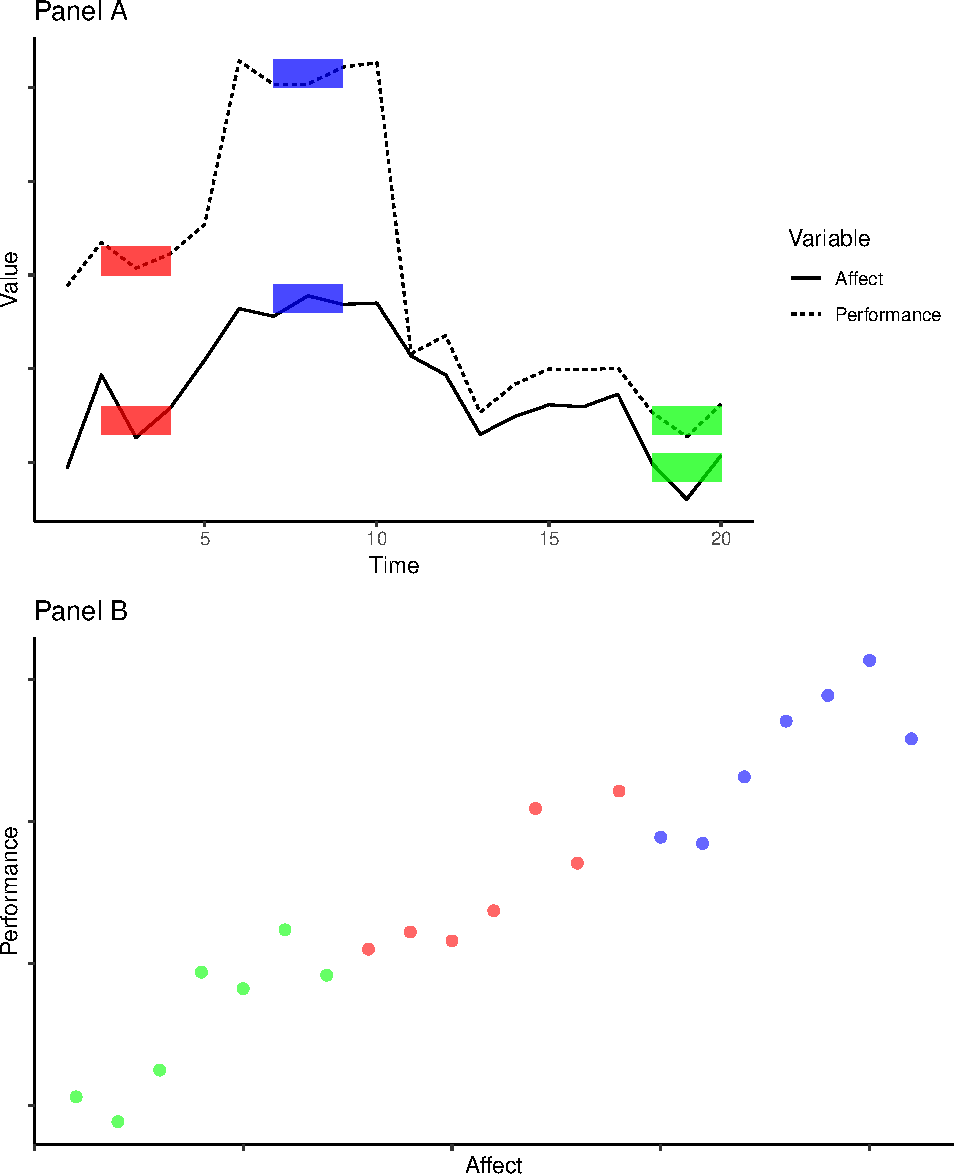
\includegraphics{figures/unnamed-chunk-17-1.pdf}
\caption{\label{fig:unnamed-chunk-17}Relating affect to performance on one
unit across time.\label{relation_ts}}
\end{figure}

\begin{figure}
\centering
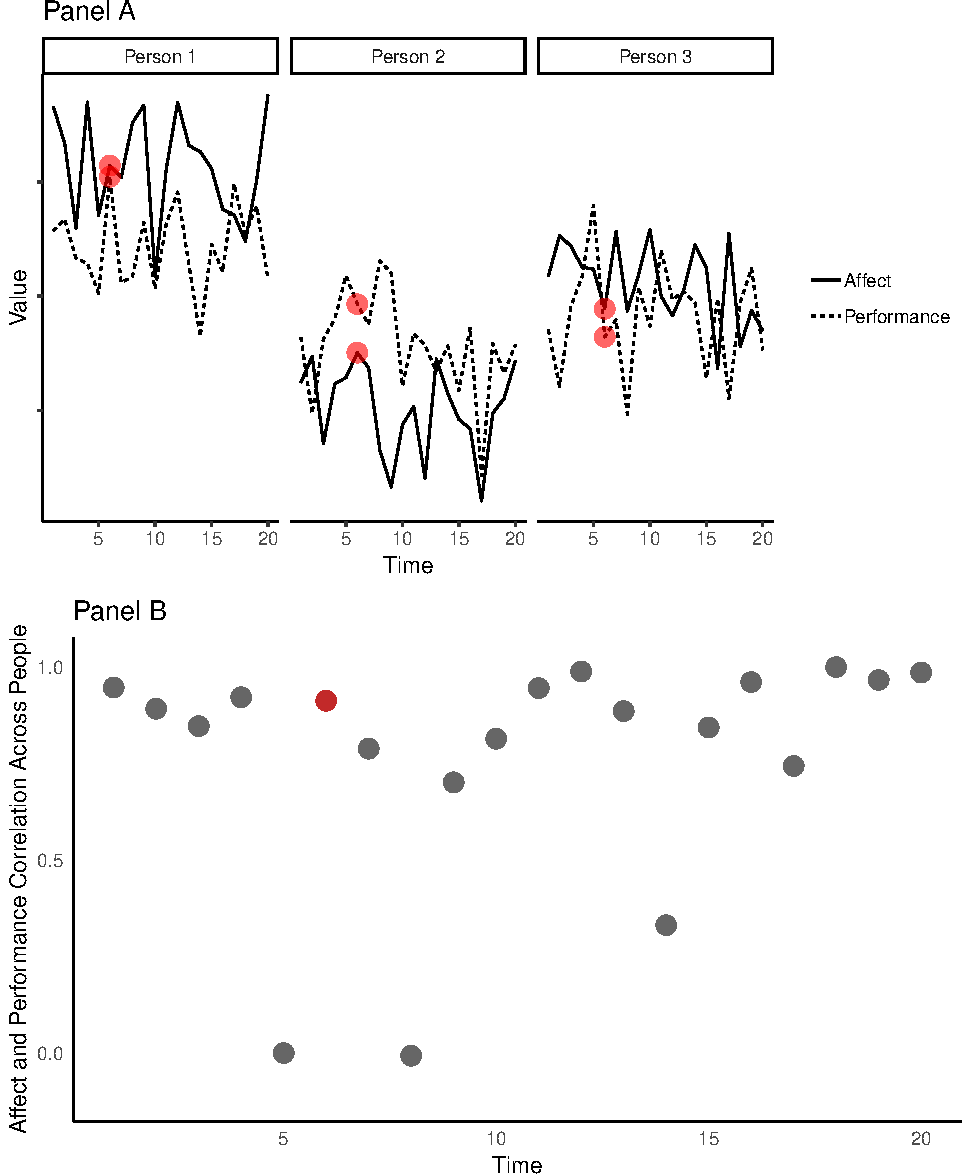
\includegraphics{figures/unnamed-chunk-18-1.pdf}
\caption{\label{fig:unnamed-chunk-18}Relating affect to performance across
units over time. The red circles demonstrate the between unit
correlation for time point six. A typical time-varying covariates model
constrains the correlation to be equivalent across time. Here, the
relationship is unconstrained at each time point.\label{relation_tvc}}
\end{figure}

\hypertarget{dynamics}{%
\section{Dynamics}\label{dynamics}}

Dynamics refers to a specific branch of mathematics, but the term is
used in different ways throughout our literature. It is used informally
to mean \enquote{change}, \enquote{fluctuating,} \enquote{volatile,}
\enquote{longitudinal,} or \enquote{over time} (among others), whereas
formal definitions in our literature are presented within certain
contexts. Wang (2016) defines a dynamic \emph{model} as a
\enquote{representation of a system that evolves over time. In
particular it describes how the system evolves from a given state at
time \emph{t} to another state at time \emph{t + 1} as governed by the
transition rules and potential external inputs} (p.~242). Vancouver,
Wang, and Li (2018) state that dynamic \emph{variables} \enquote{behave
as if they have memory; that is, their value at any one time depends
somewhat on their previous value} (p.~604). Finally, Monge (1990)
suggests that in dynamic \emph{analyses}, \enquote{it is essential to
know how variables depend upon their own past history} (p.~409).

The crucial notion to take from dynamics, then, is memory. When the past
matters, and future states are constrained by where they were at prior
points in time, dynamics are at play. In this section, we unpack a
variety of inferences that are couched in this idea.

Does performance relate to itself over time? Do current helping
behaviors depend on prior helping behaviors? Does unit climate
demonstrate self-similarity across time? Does income now predict income
in the future? These are questions about the relationship of a single
variable with itself over time -- does it predict itself at each
subsequent moment? Is it constrained by where it was in the past?

Panel A of figure \ref{dynamics_figure} shows the concept with a box and
arrow diagram. \(x\) predicts itself across every moment -- it has
self-similarity and its value now is constrained by where it was a
moment ago. In our diagram we show that \(x\) at time \(t\) is related
to \(x\) at time \(t + 1\). In other words, we posit that \(x\) shows a
lag-one relationship, where \(x\) is related to its future value one
time step away. Modelers and theorists are of course free to suggest any
lag amount that they believe captures the actual relationship.

\begin{quote}
\begin{quote}
\textbf{Inference 1:} There is self-similarity in \(x\); \(x\) relates
to itself across time.
\end{quote}
\end{quote}

\begin{center}

------------

Insert Figure \ref{dynamics_figure} about here

------------

\end{center}

Inference one was about a single variable, and in the level and trend
inference sections we saw that when we moved to multiple variables we
started asking how variables relate to one another at \(t\), or at an
average window of \(t\), or across \(t\). With dynamics, where memory is
a fundamental concept, we instead ask how variables relate to one
another at different lags. Does affect predict subsequent performance?
Do prior counterproductive work behaviors relate to current incivility?
When goal discrepancy is large is effort at the subsequent time point
high? When prior depletion is low, is current emotional exhaustion high?

We can capture this second inference by relating current values on one
variable to future values on another. Equivalently, we can relate prior
values on one variable to current values on another. Panel B of figure
\ref{dynamics_figure} shows this second dynamics inference. \(x\) still
shows self-similarity across time, but it now predicts \(y\) at the
subsequent moment. We are positing a lag-one relationship between \(x\)
and \(y\). Said formally, we believe that \(x_t\) is related to
\(y_{t+1}\) (or equivalently, \(x_{t-1}\) is related to \(y_{t}\)).
Relating current to future (or prior to current) values from one
variable to another is called a \enquote{cross lag} relationship.

\begin{quote}
\begin{quote}
\textbf{Inference 2:} There is a cross-lag relationship, where one
variable relates to another at a different point in time.
\end{quote}
\end{quote}

Inference two tells us whether the patterns in one variable co-occur
with the patterns in another at a subsequent time point. Across time,
when affect is low is subsequent performance also low? A related
question is as follows: across time, when affect is low does performance
increase or decrease? This second question is about change. How does one
variable relate to the change in another?

When goal discrepancy is large does effort increase or decrease? When
unit climate is low do perceptions of the leader change? When
performance is high does self efficacy go up or down?

All of these questions are about change, but notice that change can be
construed across different lags. Change from what? Baseline? The prior
time point? The last three time points? Typically change is construed
with respect to the last time point. When affect is low, does
performance from the last to the current time point increase or
decrease? How does effort change from the prior to the current time
point when goal discrepancy is high?

Panel C of figure \ref{dynamics_figure} demonstrates this idea. We are
positing the same self-similarity in \(x\) and the same cross-lag
relationship that we saw before, but now \(y\) also has self-similarity
across time. The cross-lag relationship, therefore, is now capturing how
\(y\) has changed from the last point in time.

It is typical to think of change from the prior to the current time
point, but researchers are free to move it as they please. Here are the
two final inferences that capture change in different locations.

\begin{quote}
\begin{quote}
\textbf{Inference 3:} There is a change relationship, where one variable
relates to the change in another.
\end{quote}
\end{quote}

\begin{quote}
\begin{quote}
\textbf{Inference 4:} There is a cross-lag relationship of change, where
one variable relates to the change of another at a different point in
time.
\end{quote}
\end{quote}

\hypertarget{dynamics-inference-table}{%
\subsection{Dynamics Inference Table}\label{dynamics-inference-table}}

We provide an inference table below -- this time with respect to dynamic
inferences. Inference one is about autoregression, or memory in a single
variable. Inference two asks how a variable at one time co-occurs with
another at a different time. Inferences three and four focus on change:
when one variable is high or low, does it relate to the change (an
increase or decrease) in the values of another variable?

\begin{center}

------------

Insert Table \ref{dynamics_table} about here

------------

\end{center}

\hypertarget{extensions}{%
\subsection{Extensions}\label{extensions}}

We described a simple set of inferences above, but the ideas generalize
to more complex dynamics as well. Often researchers are interested in
reciprocal relationships, where \(x\) influences subsequent \(y\), which
then goes back to influence \(x\) at the next time point. Said formally,
\(x_t\) influences \(y_{t+1}\), which then influences \(x_{t+2}\). Said
informally, current performance influences subsequent self-efficacy,
which then influences performance on the next trial. These inferences
are no different than what we saw above -- they are cross-lag
predictions -- all we did here was add more of them. Panel D of figure
\ref{dynamics_figure} shows reciprocal dynamics, where both \(x\) and
\(y\) show self-similarity and cross-lag relationships with one another.

The dynamic inferences shown here also generalize to systems of
variables, where a researcher posits self-similarity and cross-lag
predictions across many variables. There could be reciprocal dynamics
between a set of variables like performance, self-efficacy, and affect.
There could be a sequence of influence where initial dyadic exchanges
influence subsequent team perceptions, which then influences later
performance, and performance changes the structure of task which
ultimately initiates new dyadic exchanges. Once a researcher grasps the
foundational ideas presented here he or she is free to explore any
number of complex relationships.

Also notice that complex dynamics subsume the concept of mediation. It
is of course an important idea, but when we focus on systems of
variables and reciprocal dynamics we place our emphasis elsewhere. If
readers are interested in mediation we urge them to read one of the many
great papers on it (Maxwell \& Cole, 2007; Maxwell, Cole, \& Mitchell,
2011; Stone-Romero \& Rosopa, 2008).

\hypertarget{models-3}{%
\subsection{Models}\label{models-3}}

There are a number of recent papers on dynamic modeling that cover the
inferences discussed in this section. Wang et al. (2016) reviews many
different types of dynamic models and, although his paper will not
provide readers will specific code it is an excellent starting paper to
observe the variety of models available. When a researcher wants to
explore dynamic inferences with respect to a single unit over time they
will be examining time-series data, and there are a number of models for
this application. DeShon (2012) discusses autoregressive distributed lag
(ARDL) and vector autoregressive models, and Jebb and collegues (2017;
2015) introduce ARDL and autoregressive distributed moving average
(ARIMA) models. Finally, Xu and DeShon (almost) discuss a dynamic model
first introduced by Bollen and Brand (2010). This dynamic panel model is
appropriate for researchers who want to model dynamics across more than
one unit. Moreover, it is better suited than HLM for typical situations
in organizational psychology and management (i.e., short \(t\) and large
\(N\)).

\begin{table}

\caption{\label{tab:unnamed-chunk-19}\label{dynamics_table}Examples of dynamic inferences.}
\centering
\begin{tabular}[t]{>{\raggedright\arraybackslash}p{5em}>{\raggedright\arraybackslash}p{30em}}
\toprule
Inference & Examples\\
\midrule
1 & Burnout demonstrates self-similarity across time.\newline Performance relates to subsequent performance.\\
\hline
2 & Affect predicts subsequent counterproductive work behaviors.\newline Turnover relates to subsequent firm performance.\\
\hline
3 & Positive health status relates to change in happiness.\newline Anxiety relates to change in performance.\\
\hline
4 & Affect relates to subsequent change in performance.\newline Helping behaviors predict subsequent depletion changes.\\
\bottomrule
\end{tabular}
\end{table}

\begin{figure}

{\centering 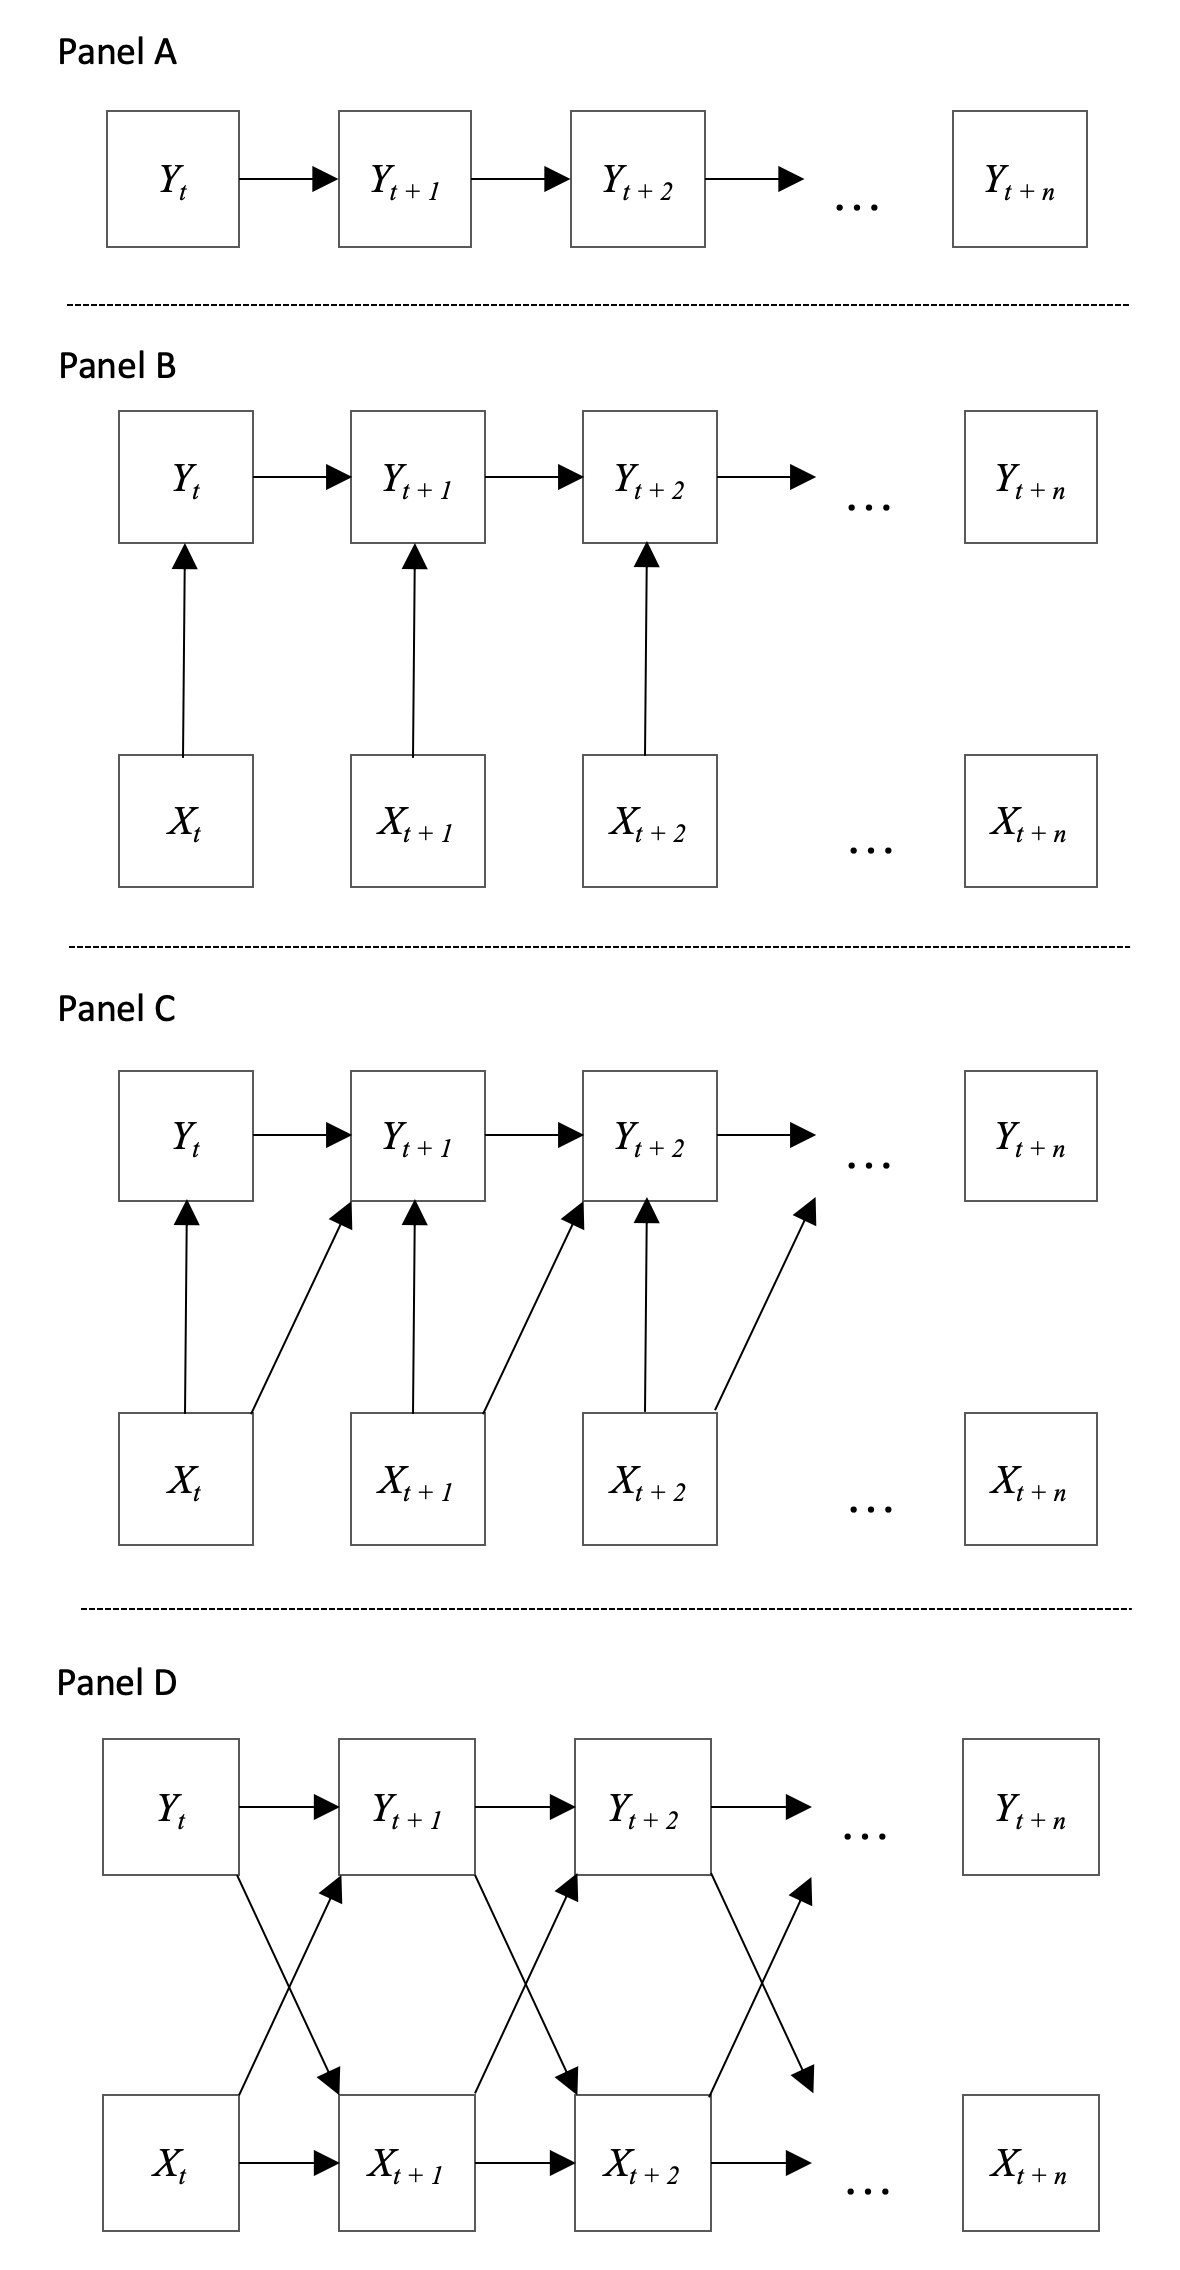
\includegraphics[width=3.75in]{figures/dynamics/dall} 

}

\caption{Univariate and bivariate dynamics adapted from DeShon (2012). Panel A shows self-similarity or autoregression in $X$ across time. Panel B shows $X$ predicting subsequent $Y$. Panel C shows $X$ predicting subsequent change in $Y$. Panel D shows reciprocal dynamics between $X$ and $Y$.\label{dynamics_figure}}\label{fig:unnamed-chunk-20}
\end{figure}

\hypertarget{discussion}{%
\section{Discussion}\label{discussion}}

There are many different patterns to explore with longitudinal data
structures. What does performance look like over time? Does it
fluctuate? Is the trajectory consistent across people? What is its
initial or ending level? Does it show a growth pattern? Does that growth
pattern covary with another trend? Does it move across time in relation
to another variable? Does it show self-similarity or memory? Does it
show lagged relationships with other variables? Is it part of a
reciprocal system? In this paper we presented a framework that organizes
these inferences into a fundamental set. We discussed what the
inferences mean, how to pose questions and hypotheses about them, and
linked the inferences to appropriate statistical models. As our field
dives into within-person, dynamic, and process-oriented methods we hope
this paper helps researchers understand the spectrum of inferences that
they can explore with rich longitudinal data.

\newpage

\hypertarget{references}{%
\section{References}\label{references}}

\setlength{\parindent}{-0.5in}
\setlength{\leftskip}{0.5in}

\hypertarget{refs}{}
\leavevmode\hypertarget{ref-barnes_lack_2011}{}%
Barnes, C. M., Schaubroeck, J., Huth, M., \& Ghumman, S. (2011). Lack of
sleep and unethical conduct. \emph{Organizational Behavior and Human
Decision Processes}, \emph{115}(2), 169--180.

\leavevmode\hypertarget{ref-beal_esm_2015}{}%
Beal, D. J. (2015). ESM 2.0: State of the art and future potential of
experience sampling methods in organizational research. \emph{Annu. Rev.
Organ. Psychol. Organ. Behav.}, \emph{2}(1), 383--407.

\leavevmode\hypertarget{ref-bliese_growth_2002}{}%
Bliese, P. D., \& Ployhart, R. E. (2002). Growth modeling using random
coefficient models: Model building, testing, and illustrations.
\emph{Organizational Research Methods}, \emph{5}(4), 362--387.

\leavevmode\hypertarget{ref-bollen_general_2010}{}%
Bollen, K. A., \& Brand, J. E. (2010). A general panel model with random
and fixed effects: A structural equations approach. \emph{Social
Forces}, \emph{89}(1), 1--34.

\leavevmode\hypertarget{ref-chi_can_2015}{}%
Chi, N.-W., Chang, H.-T., \& Huang, H.-L. (2015). Can personality traits
and daily positive mood buffer the harmful effects of daily negative
mood on task performance and service sabotage? A self-control
perspective. \emph{Organizational Behavior and Human Decision
Processes}, \emph{131}, 1--15.

\leavevmode\hypertarget{ref-deshon_multivariate_2012}{}%
DeShon, R. P. (2012). Multivariate dynamics in organizational science.
\emph{The Oxford Handbook of Organizational Psychology}, \emph{1},
117--142.

\leavevmode\hypertarget{ref-dunford_is_2012}{}%
Dunford, B. B., Shipp, A. J., Boss, R. W., Angermeier, I., \& Boss, A.
D. (2012). Is burnout static or dynamic? A career transition perspective
of employee burnout trajectories. \emph{Journal of Applied Psychology},
\emph{97}(3), 637--650.
doi:\href{https://doi.org/http://dx.doi.org.proxy2.cl.msu.edu/10.1037/a0027060}{http://dx.doi.org.proxy2.cl.msu.edu/10.1037/a0027060}

\leavevmode\hypertarget{ref-finch2016multilevel}{}%
Finch, W. H., Bolin, J. E., \& Kelley, K. (2016). \emph{Multilevel
modeling using r}. Crc Press.

\leavevmode\hypertarget{ref-grimm_growth_2016}{}%
Grimm, K. J., Ram, N., \& Estabrook, R. (2016). \emph{Growth modeling:
Structural equation and multilevel modeling approaches}. Guilford
Publications.

\leavevmode\hypertarget{ref-hulsheger_dawn_2016}{}%
Hülsheger, U. R. (2016). From dawn till dusk: Shedding light on the
recovery process by investigating daily change patterns in fatigue.
\emph{Journal of Applied Psychology}, \emph{101}(6), 905--914.
doi:\href{https://doi.org/http://dx.doi.org.proxy2.cl.msu.edu/10.1037/apl0000104}{http://dx.doi.org.proxy2.cl.msu.edu/10.1037/apl0000104}

\leavevmode\hypertarget{ref-ilgen_computational_2000}{}%
Ilgen, D. R., \& Hulin, C. L. (2000). \emph{Computational modeling of
behavior in organizations: The third scientific discipline.} American
Psychological Association.

\leavevmode\hypertarget{ref-jebb_introduction_2017}{}%
Jebb, A. T., \& Tay, L. (2017). Introduction to time series analysis for
organizational research: Methods for longitudinal analyses.
\emph{Organizational Research Methods}, \emph{20}(1), 61--94.

\leavevmode\hypertarget{ref-jebb_time_2015}{}%
Jebb, A. T., Tay, L., Wang, W., \& Huang, Q. (2015). Time series
analysis for psychological research: Examining and forecasting change.
\emph{Frontiers in Psychology}, \emph{6}, 727.

\leavevmode\hypertarget{ref-kozlowski_work_2003}{}%
Kozlowski, S. W., \& Bell, B. S. (2003). Work groups and teams in
organizations. \emph{Handbook of Psychology}, 333--375.

\leavevmode\hypertarget{ref-maxwell2007bias}{}%
Maxwell, S. E., \& Cole, D. A. (2007). Bias in cross-sectional analyses
of longitudinal mediation. \emph{Psychological Methods}, \emph{12}(1),
23.

\leavevmode\hypertarget{ref-maxwell2011bias}{}%
Maxwell, S. E., Cole, D. A., \& Mitchell, M. A. (2011). Bias in
cross-sectional analyses of longitudinal mediation: Partial and complete
mediation under an autoregressive model. \emph{Multivariate Behavioral
Research}, \emph{46}(5), 816--841.

\leavevmode\hypertarget{ref-mcardle_latent_1987}{}%
McArdle, J. J., \& Epstein, D. (1987). Latent Growth Curves within
Developmental Structural Equation Models. \emph{Child Development},
\emph{58}(1), 110--133.
doi:\href{https://doi.org/10.2307/1130295}{10.2307/1130295}

\leavevmode\hypertarget{ref-monge_theoretical_1990}{}%
Monge, P. R. (1990). Theoretical and analytical issues in studying
organizational processes. \emph{Organization Science}, \emph{1}(4),
406--430.

\leavevmode\hypertarget{ref-pitariu_explaining_2010}{}%
Pitariu, A. H., \& Ployhart, R. E. (2010). Explaining change: Theorizing
and testing dynamic mediated longitudinal relationships. \emph{Journal
of Management}, \emph{36}(2), 405--429.

\leavevmode\hypertarget{ref-ployhart_longitudinal_2010}{}%
Ployhart, R. E., \& Vandenberg, R. J. (2010). Longitudinal research: The
theory, design, and analysis of change. \emph{Journal of Management},
\emph{36}(1), 94--120.

\leavevmode\hypertarget{ref-schonfeld2007hierarchical}{}%
Schonfeld, I. S., \& Rindskopf, D. (2007). Hierarchical linear modeling
in organizational research: Longitudinal data outside the context of
growth modeling. \emph{Organizational Research Methods}, \emph{10}(3),
417--429.

\leavevmode\hypertarget{ref-singer_applied_2003}{}%
Singer, J. D., Willett, J. B., \& Willett, J. B. (2003). \emph{Applied
longitudinal data analysis: Modeling change and event occurrence}.
Oxford university press.

\leavevmode\hypertarget{ref-stone2008relative}{}%
Stone-Romero, E. F., \& Rosopa, P. J. (2008). The relative validity of
inferences about mediation as a function of research design
characteristics. \emph{Organizational Research Methods}, \emph{11}(2),
326--352.

\leavevmode\hypertarget{ref-vancouver_translating_2018}{}%
Vancouver, J. B., Wang, M., \& Li, X. (2018). Translating Informal
Theories Into Formal Theories: The Case of the Dynamic Computational
Model of the Integrated Model of Work Motivation. \emph{Organizational
Research Methods}, 109442811878030.
doi:\href{https://doi.org/10.1177/1094428118780308}{10.1177/1094428118780308}

\leavevmode\hypertarget{ref-Wang2016}{}%
Wang, M., Zhou, L., \& Zhang, Z. (2016). Dynamic modeling. \emph{Annual
Review of Organizational Psychology and Organizational Behavior},
\emph{3}(1), 241--266.
doi:\href{https://doi.org/10.1146/annurev-orgpsych-041015-062553}{10.1146/annurev-orgpsych-041015-062553}


\end{document}
